\documentclass{beamer}
\usetheme{Boadilla}
\usecolortheme{default}
\usepackage{graphicx}
\usepackage[spanish]{babel}

\title{Ventas de videojuegos}
\subtitle{Un análisis en las ventas de más de 16500 juegos}
\author{Equipo SSSE}
%% \date{\today}
\begin{document}
	\begin{frame}
		\maketitle
	\end{frame}
	
	\begin{frame}{Puntos a tratar}
		\tableofcontents
	\end{frame}
	
	\section{Contexto}
	\begin{frame}[t]{Contexto}
		El equipo decide trabajar con un conjunto de datos desconocido pero que despierta pasión en el equipo: \textbf{Videojuegos}. Se trabajan con las siguientes características:
		\begin{itemize}
			\item Datos desde el 2000 al 2017
			\item Plataformas de videojuegos tradicionales, pero no se incluye smartphones.
			\item Información por regiones en base a la definición de Sony de regiones globales*
		\end{itemize}
	\end{frame}
	
	\section{Consolas}
	\begin{frame}[t]{Consolas}
		\begin{figure}
			\centering
			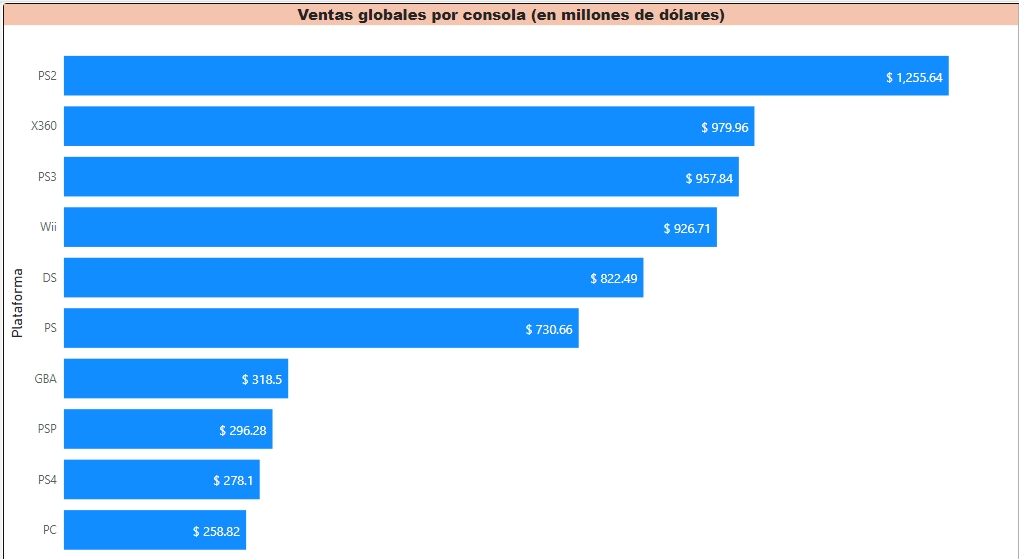
\includegraphics[width=4.2in]{m1.png}
			\caption{Ventas por consola}
		\end{figure}
	\end{frame}
	
	\section{Plataformas por año}
	\begin{frame}{Plataformas por año}
		\begin{figure}
			\centering
			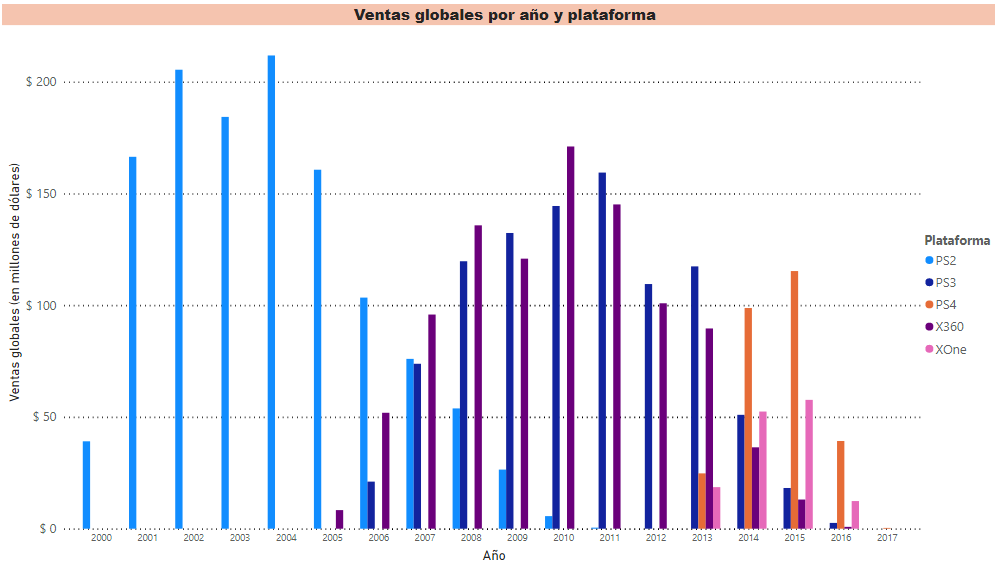
\includegraphics[width=4.2in]{m2.png}
			\caption{Consolas en el tiempo}
		\end{figure}
	\end{frame}
	
	\section{Región y género}
	\begin{frame}{Región y género}
		\begin{figure}
			\centering
			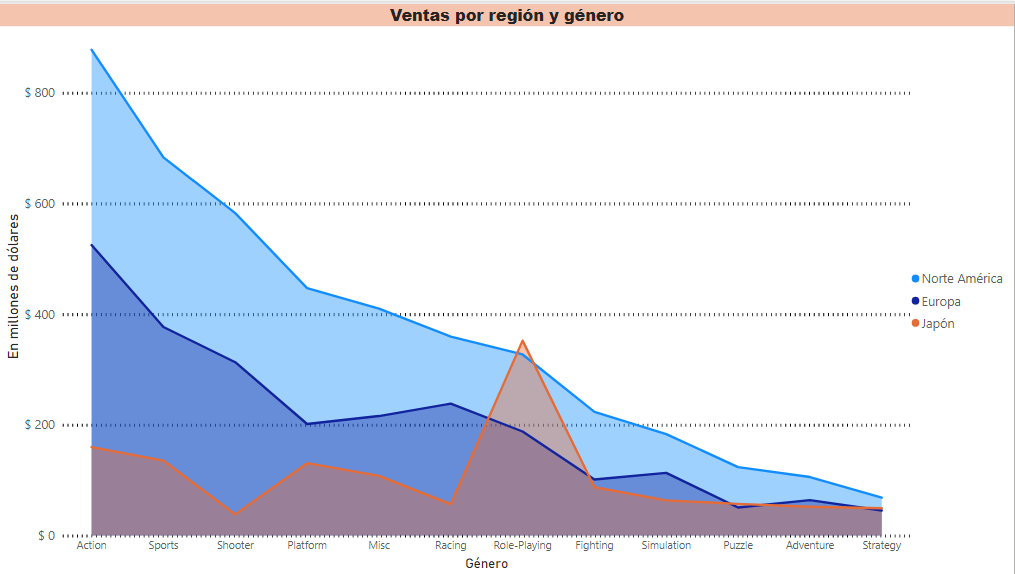
\includegraphics[width=4.2in]{m3.png}
			\caption{Regiones y género}
		\end{figure}
	\end{frame}
	
\end{document}